\documentclass{cmspaper}
\begin{document}

%==============================================================================
% title page for few authors

\begin{titlepage}

% select one of the following and type in the proper number:
   \cmsnote{2008/000}
%  \internalnote{2005/000}
%  \conferencereport{2005/000}
   \date{23 July 2008}

  \title{Photon Identification for CMS Startup}

  \begin{Authlist}
    A.~Askew, O.~Atramentov, Y.~Gershtein,
       \Instfoot{FSU}{Florida State University, Tallahassee, FL.}

    A.~Debenedetti,
	\Instfoot{Minn}{University of Minnesota, Minneapolis, MN.}

    M.~Gataullin, V.~Litvin, J.~Veverka, 
	\Instfoot{CalTech}{California Institute of Technology, Pasadena, CA.}

    T.~Miceli, J.~Stilley,
	\Instfoot{UCDavis}{University of California at Davis, Davis, CA.}

    V.~Gaultney,
        \Instfoot{FIU}{Florida International University, Miami, FL.}

    S.~Shrestha,
        \Instfoot{KSU}{Kansas State University, Manhattan, KS.}

    M.~Anderson
        \Instfoot{Wisc}{University of Wisconsin, Madison, WI.}

  \end{Authlist}

% if needed, use the following:
%\collaboration{Flying Saucers Investigation Group}
%\collaboration{CMS collaboration}

  \begin{abstract}
This note defines the methods by which the identification of photons may be verified from data
on start up.  This verification includes measurement of the photon efficiency, as well as methods
for obtaining photon purity.  Backgrounds to photons from jets and electrons are discussed, and an
example set of ``vanilla'' photon identification requirements are presented. 
  \end{abstract} 

% if needed, use the following:
%\conference{Presented at {\it Physics Rumours}, Coconut Island, April 1, 2005}
%\submitted{Submitted to {\it Physics Rumours}}
%\note{Preliminary version}
  
\end{titlepage}

\setcounter{page}{2}%JPP

\section{Introduction}
Photon identification at hadron colliders is a difficult task, mainly due to the large backgrounds from hadronic jets and
the lack of a di-photon signal resonance for studies.  This difficulty is further compounded by the fact that unlike electrons,
photons are not redundant
\footnote{Unconverted photons are not redundant.  For the special case of conversions with reconstructed
tracks, please see~\cite{NancyConv}.}, e.g. they leave a signal in only one detector, the electromagnetic calorimeter.  Thus photons are subject to backgrounds (such as cosmic/halo muon bremsstrahlung) which do not typically afflict electrons.
Worse, direct studies of photons for the purposes of determining efficiencies in the data are not possible for small amounts of integrated luminosity.  This is mitigated somewhat by the reconstruction of photons in $Z\gamma\rightarrow\ell\ell\gamma$ events in which the photon is radiated off one of the final state leptons.

For early (small) samples of integrated luminosity, one appeals to electrons to give information about relevant reconstruction quantities, for shower shape and isolation quantities.  It will be shown that for proper selection of analysis quantities, one may use the electrons from $Z\rightarrow ee$ to provide measurements of photon efficiencies, as well as templates for the determination of the purity in photon samples.  These efficiencies can then be (to the limit of available statistics) verified with early samples of $Z\gamma\rightarrow\ell\ell\gamma$.  Special tags are also developed to allow for the study of cosmic and beam halo muon events. 

\section{Photon Reconstruction and LooseEM}
In order to utilize the flexibility of the photon reconstruction software, a base definition {\bf LooseEM} is defined to provide a starting point for both signal and background studies\footnote{There is a software delineation between the EgammaPhotonProducer package, which constructs the actual reco::Photon, and the PhotonIdentification package which is mainly concerned with the organization and analysis of reco::Photon objects.  The interested reader is referred to Appendix B.}.  The object of the {\bf LooseEM} definition is to provide a definition of objects that are reconstructed as photons which are 100\% efficient for true photons (produced in collisions), but still provides some rejection against fake photons from hadronic activity.  A {\bf LooseEM} for the purposes of this documents is defined as a reco::Photon which meets the following criteria:
\begin{list}{$\bullet$}
 \item{The reco::Photon must be isolated from other deposits of energy in the ECAL.  The sum of the energy deposited in a cone
of $\Delta R <$0.4 minus the energy that is clustered into the photon must be smaller than 20~GeV.  This threshold may seem high (the distribution is presented in Figure~\ref{fig:EMiso_EMLoose}), realize that this is due to the fact that no threshold (except for $E_{crys} >$ 0 GeV) is applied to the hits considered.}
 \item{The reco::Photon must be isolated from surrounding deposits of energy in the HCAL.  The sum of the energy in the HCAL in
a hollow cone of 0.1 $< \Delta R<$0.4 is required to be smaller than 10~GeV.  As mentioned in the above point, no threshold save that the cells are above 0 GeV is applied.  Note that the selection of this hollow cone is to make the measurement of this isolation quantity independent of the calculation of the hadronic-electromagnetic energy ratio.}
 \item{The reco::Photon is required to have its $HadOverEM$ ratio be smaller than 0.2.  $HadOverEM$ here is defined as the energy within $\Delta R=$0.1 of the supercluster centroid in the hadronic calorimeter divided by the energy of the supercluster.  As of the writing of this note (which stands astride software versions 2\_0 and 2\_1) this cut will become the default in the photon reconstruction used for startup.  Since the distributions shown depend on the earlier version of the reconstruction, this requirement can be shown to be very efficient for photons, and well in line with the philosophy of LooseEM selection.}
\end{list}
Distributions of each of these quantities are shown for nominal samples of signal and background in Figures~\ref{fig:EMiso_EMLoose},~\ref{fig:HCALiso_EMLoose}, and~\ref{fig:HadOverEM_EMLoose}.  All of these distributions are shown for barrel photons only, and here, this document will concentrate explicitly on barrel only since these will be available at startup.
\begin{figure}[hbtp]
  \begin{center}
    \resizebox{10cm}{10cm}{\includegraphics{EMLoose/EMiso_EMLoose.eps}}
    \caption{ECAL isolation energy for direct photons (blue) and for fakes from dijets (red).}
    \label{fig:EMiso_EMLoose}
  \end{center}
\end{figure}
\begin{figure}[hbtp]
  \begin{center}
    \resizebox{10cm}{10cm}{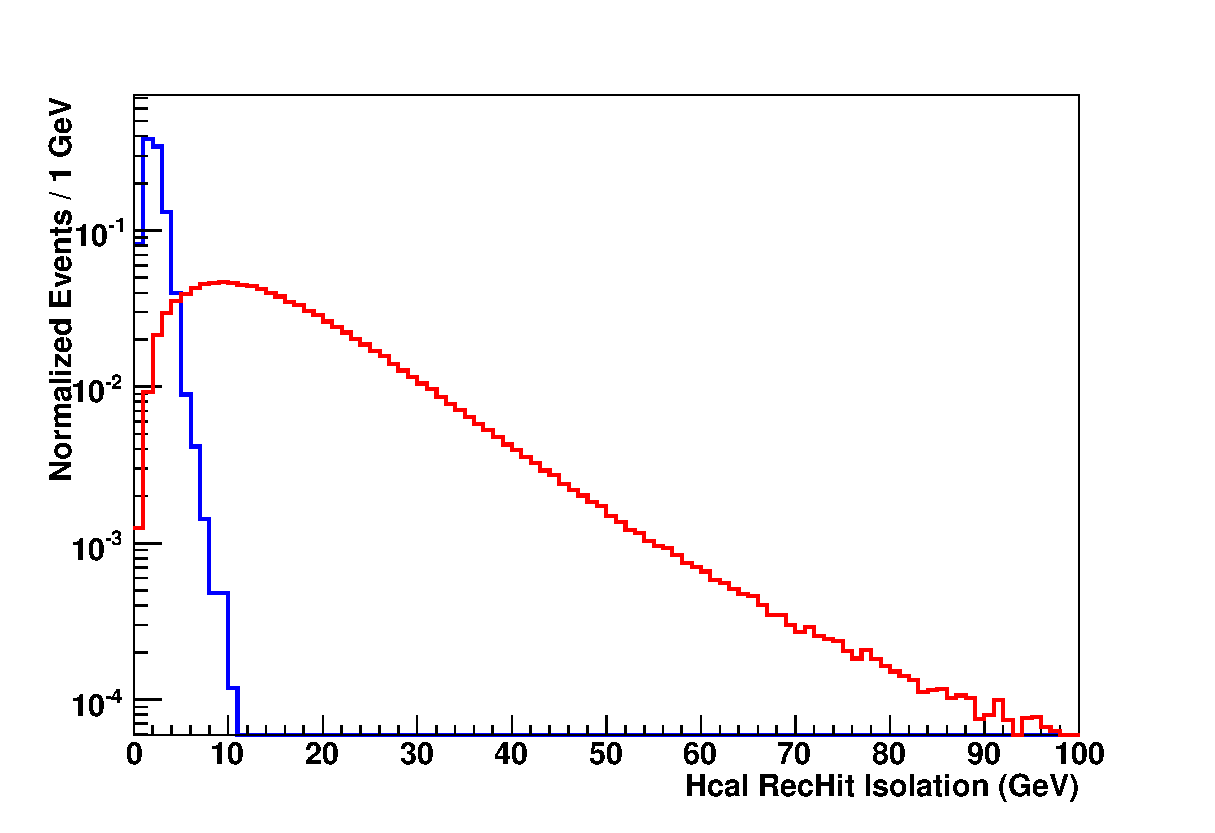
\includegraphics{EMLoose/HCALiso_EMLoose.eps}}
    \caption{HCAL isolation energy for direct photons (blue) and for fakes from dijets (red).}
    \label{fig:HCALiso_EMLoose}
  \end{center}
\end{figure}
\begin{figure}[hbtp]
  \begin{center}
    \resizebox{10cm}{10cm}{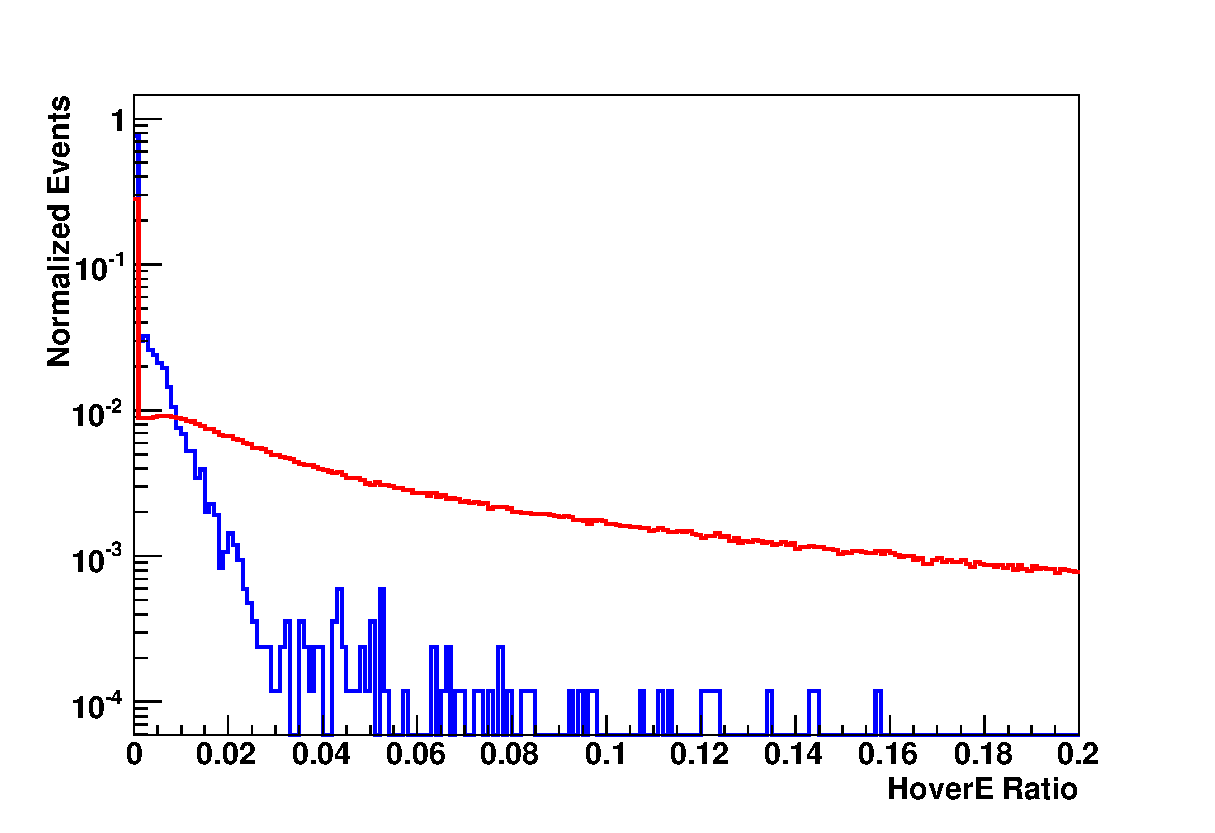
\includegraphics{EMLoose/HadOverEM_EMLoose.eps}}
    \caption{HadOverEM ratio for direct photons (blue) and for fakes from dijets (red).}
    \label{fig:HadOverEM_EMLoose}
  \end{center}
\end{figure}
The signal sample shown here is a sample of QCD direct photon production produced privately in CMSSW\_2\_1\_0\_pre5, in which the generated photon was required to match to a reconstructed reco::Photon object.  The background sample was a sample of inclusive QCD dijets which were produced in the official CSA08 production, which made use of CMSSW\_2\_0\_5.  As previously mentioned, only barrel photons are considered here, and further, the photon $E_{T}$ is required to be greater than 20~GeV.
As one can see, these cuts remove a significant portion of the jet background, while retaining most if not all of the true photons.  The efficiency of these cuts, and their measurement from the data is discussed in Section~\ref{ssec:LooseEMEff}.

\section{Photon Identification Quantities and Selection}
With the base {\bf LooseEM} definition in place, more specific selection cuts for photon identification may be chosen.  Two additional definitions are made here {\bf LoosePhoton} and {\bf TightPhoton}.  
A {\bf LoosePhoton} is defined as a {\bf LooseEM} with:
\begin{list}{$\bullet$}
 \item{$HadOverEM$ ratio of smaller than 0.1.}
\item{Isolation from electromagnetic activity (as defined in {\bf LooseEM}) smaller than 15 GeV.}
\item{The sum of the $p_{T}$ of tracks within a hollow cone of $\Delta R<$(0.4-0.0X) is required to be smaller than 5 GeV.}
\end{list}
A {\bf TightPhoton} satisfies all of the cuts from the {\bf LoosePhoton}, but with the additional requirement that its R9 variable (defined in Eqn.~\ref{eqn:R9}) is greater than 0.8.
\begin{equation}
 R9 = \frac{E_{3x3}}{E_{supercluster}}
\end{equation}\label{eqn:R9}
\begin{figure}[hbtp]
  \begin{center}
    \resizebox{10cm}{10cm}{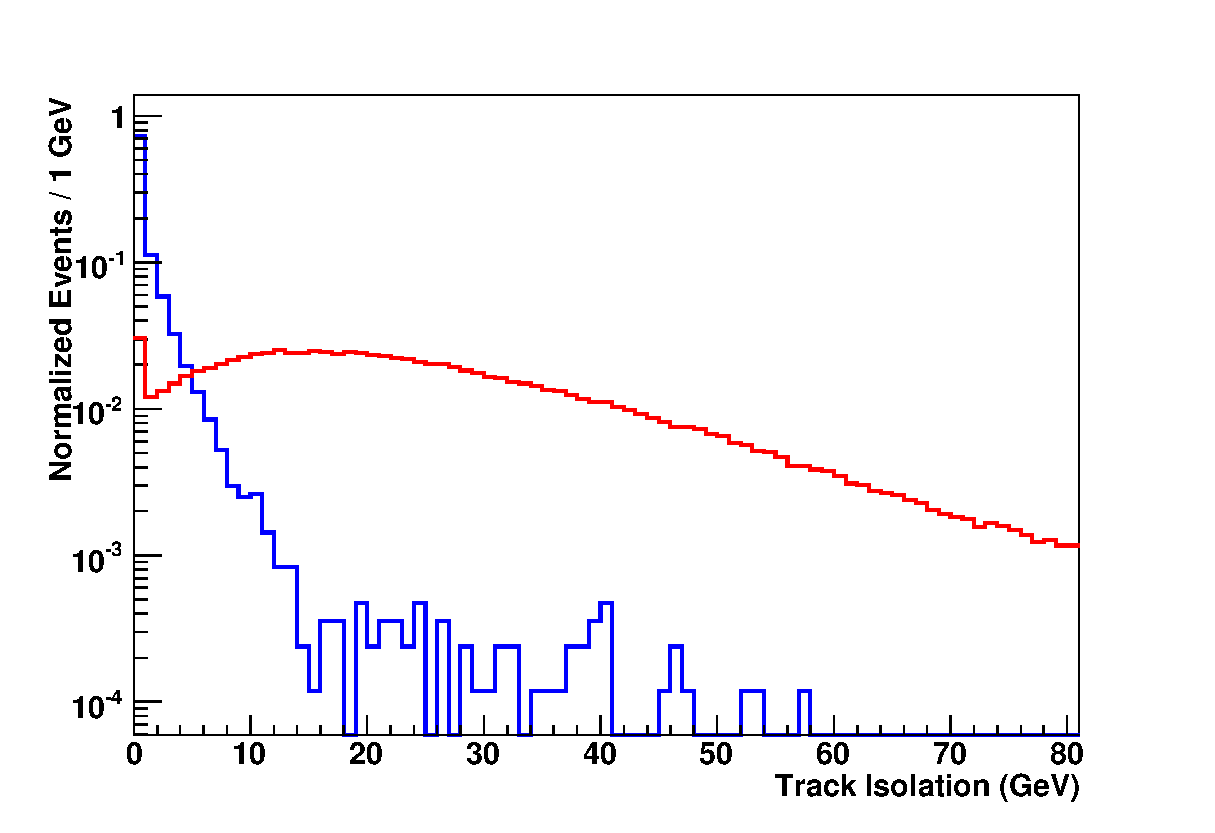
\includegraphics{PhotonSel/Photonid_trkiso.eps}}
    \caption{Sum of track $p_T$ as defined in {\bf LoosePhoton} for {\bf LooseEM} objects in direct photon events (blue) and fakes
from dijets(red).}
    \label{fig:Photonid_trkiso}
  \end{center}
\end{figure}
\begin{figure}[hbtp]
  \begin{center}
    \resizebox{10cm}{10cm}{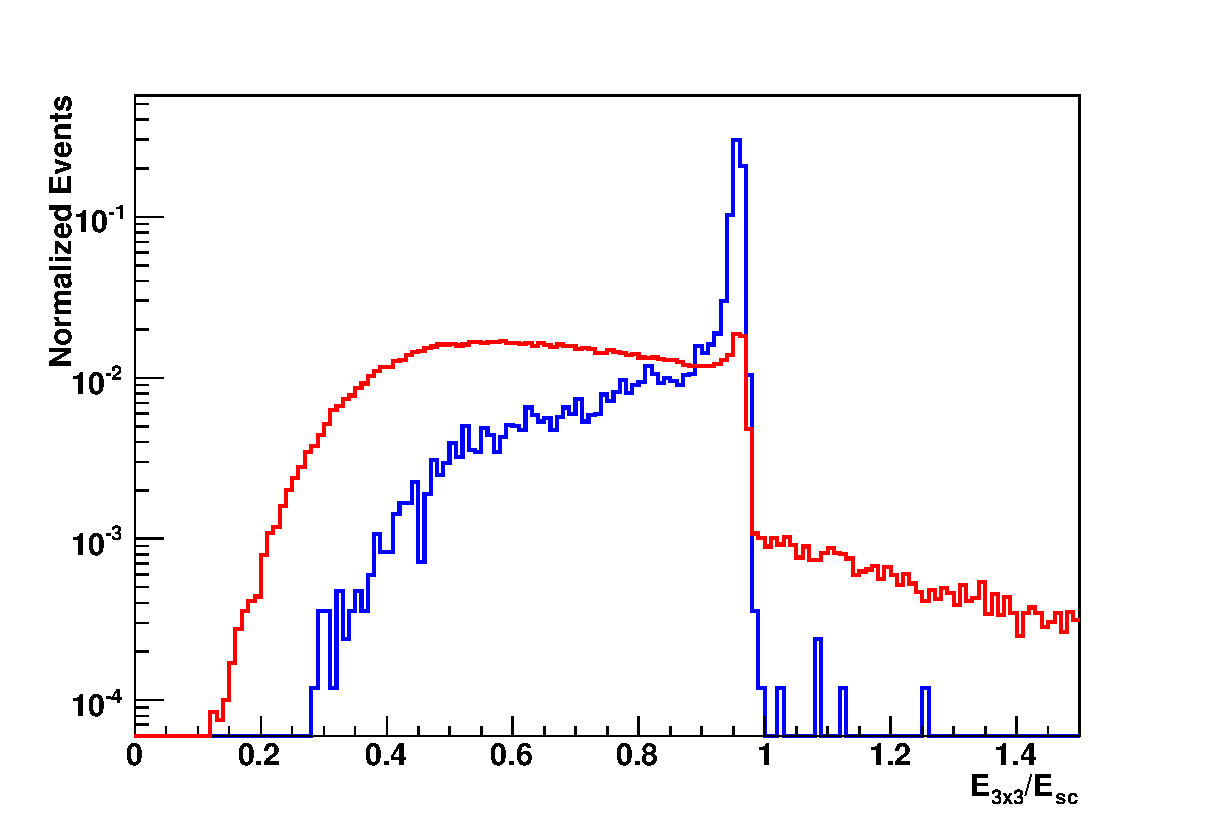
\includegraphics{PhotonSel/Photonid_r9.eps}}
    \caption{R9 variable for {\bf LooseEM} objects in direct photon events (blue) and for fakes from dijets (red).}
    \label{fig:Photonid_r9}
  \end{center}
\end{figure}

\section{Efficiency Determination in the Data}
Since photons are not redundant objects (as previously stated), the determination of the data efficiency for photon reconstruction requires more steps than the simple tag-and-probe method for electrons from $Z\rightarrow ee$ events.
The base prescription for measuring photon efficiencies in data shall be:
\begin{list}{$\bullet$}
\item{Make selection on quantities that will be as similar as possible between electrons and photons.  A good example of this is the hollow cone of the track isolation, which will be set such that for electrons the associated track will be outside this
cone such that the track isolation efficiency can be measured with electrons.}
\item{Ascertain the extent to which a cut can be made on these similar quantities.  If a cut on, say track isolation, is noticeably different between electrons and photons in the Monte Carlo, then this difference must be assigned as a systematic uncertainty.}
\item{Measure the efficiency for the given selection cuts in data using a tag-and-probe method.  Use this same tag-and-probe method to measure the efficiency in Monte Carlo, and compare with the Monte Carlo truth efficiency to check for bias.} 
\item{Scale the Monte Carlo efficiency (if necessary) to the data and calculate the final systematic uncertainty.}
\end{list}

This prescription limits one, for early data taking, to quantities that can be verified in the data from electrons.  Of course, constructing quantities that are similar for photons and electrons allows one to factorize the background somewhat, first there will be hadronic jets (which are discriminated against by the different isolation requirements), and isolated electromagnetic objects.  These electromagnetic objects, by means of a track veto, can then be separated into electrons and photons.

\subsection{LooseEM efficiency}\label{ssec:LooseEMEff}
The base {\bf LooseEM} efficiency is determined using a tag-and-probe method.  $Z$-boson events are selected first by requiring two high $p_T$ tracks, one of which is required to pass tight quality requirements and match well in $\eta-\phi$ with an electromagnetic object in the ECAL.  The second serves as a probe, and along with the cluster matched to the tag, the invariant mass can be formed, to control possible backgrounds.  The efficiency then, is the rate at which the probe track is associated with a {\bf LooseEM} object in the calorimeter.

\section{Photon Fake Rates and Purity}
\subsection{Photon-Jet Fake Rate}
\subsection{Photon-Electron Fake Rate}


\section{Additional Backgrounds to Photons}
As previously mentioned, since photons only manifest themselves as isolated clusters of energy in the electromagnetic calorimeter, they are subject to backgrounds from cosmic ray and beam halo muons which undergo bremsstrahlung in the calorimeter as they pass through.  For each of these backgrounds, one attempts to derive the contamination from these sources by identifying variables that are sensitive to the difference between these bremsstrahlung backgrounds and building templates from the data using tags.  Then along with templates from prompt electromagnetic objects in data, one can do fits to the final candidate distributions in the data to determine the final prompt fraction.

\subsection{Beam Halo Muons}
\subsection{Cosmic Ray Muons}

\begin{figure}[hbtp]
  \begin{center}
    \resizebox{10cm}{10cm}{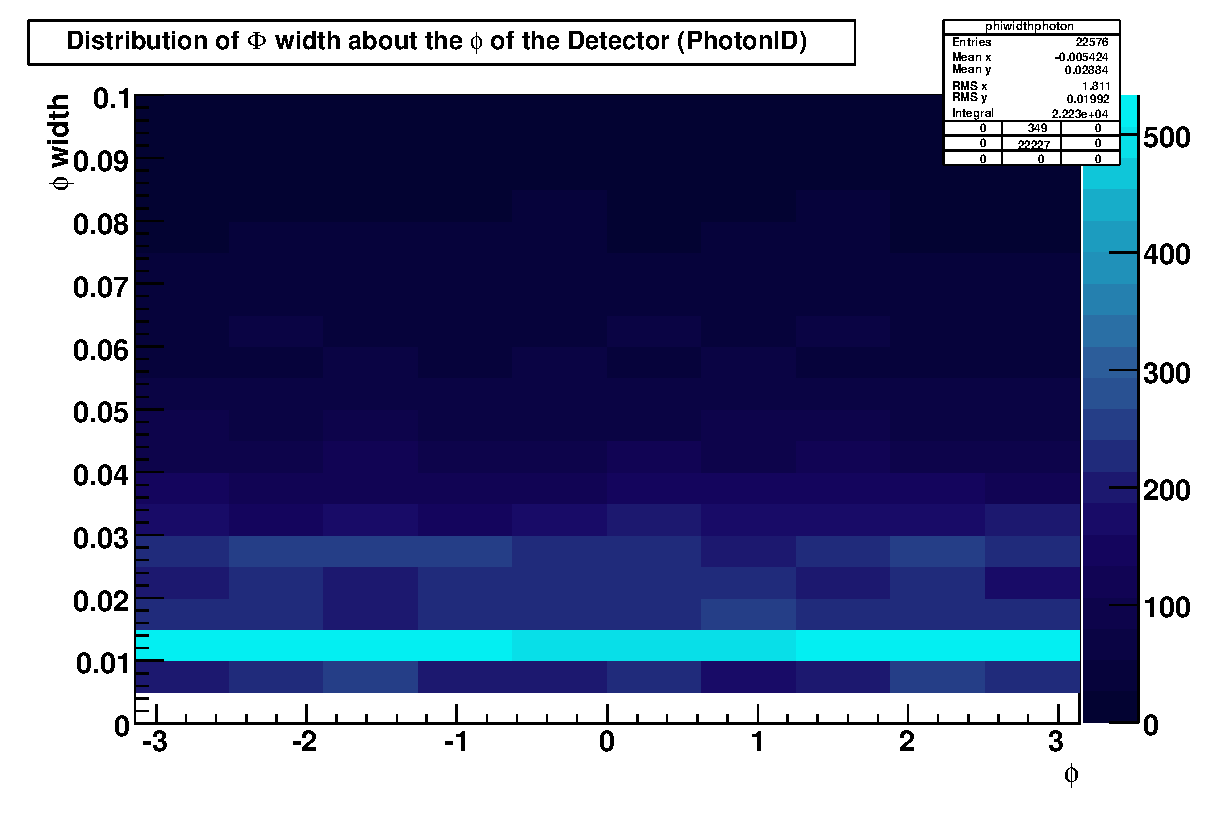
\includegraphics{CosmicPlots/photonID.eps}}
    \caption{The energy weighted width in $\phi$ as a function of detector $\phi$ for prompt, direct photons from the interaction region.  No dependence is observed.}
    \label{fig:PromptPhiWidPhi}
  \end{center}
\end{figure}

\begin{figure}[hbtp]
  \begin{center}
    \resizebox{10cm}{10cm}{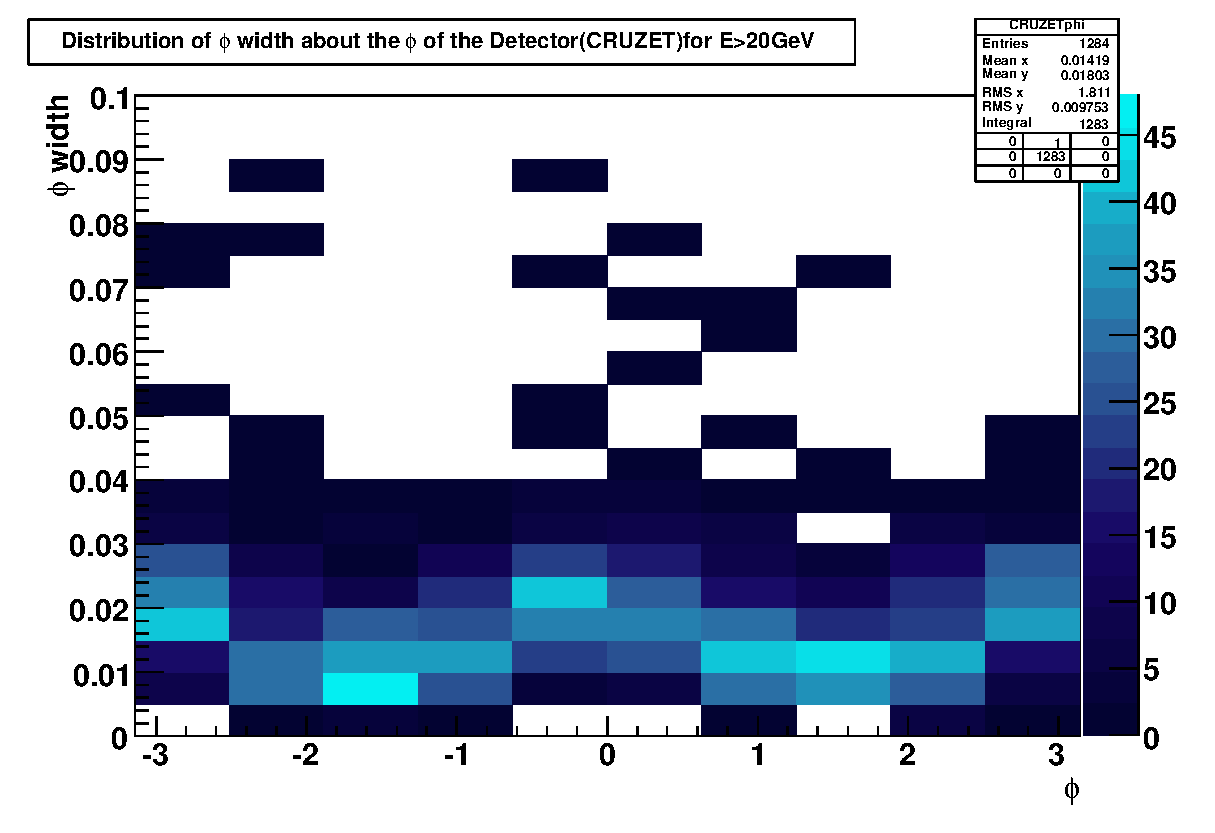
\includegraphics{CosmicPlots/CRUZET.eps}}
    \caption{The energy weighted width in $\phi$ as a function of detector $\phi$ for electromagnetic objects found in
CRUZET events.}
    \label{fig:CRUZETPhiWidPhi}
  \end{center}
\end{figure}

\section{Summary}

\begin{thebibliography}{9}
\bibitem{NancyConv}  CMSNote XXXX


\end{thebibliography}
 
%------------------------------------------------------------------------------
\pagebreak
\appendix
\section{Photon Energy Scale}

\section{Photon Software Organization and Use}

\section{Photon Identification at High Energies}

\end{document}
